\documentclass[openany]{article}
\usepackage[a4paper,margin=1in,bottom=1.5in]{geometry} % define margins. Bottom margin is used to lift a little bit the page number.
\usepackage[english]{babel} % document language is english
\usepackage{tikz} % for drawing (currently not used).
\usepackage{graphicx} % for including images
\usepackage[export]{adjustbox}
\usepackage{fancyhdr} % used for creating headers and footers. only used in title page in this document.
\usepackage{tabularx} % creation of more complex tables
\usepackage{longtable} % tables can span multiple pages
\usepackage{array} % allow elements of tabular environment to have vertical alignment, e.g., center alignment.
\usepackage{nameref} % make it possible to reference by name
\usepackage{hyperref} % allow hiperlinks (links to other document parts and extern links)
\usepackage{etoc} % used for generation of section local table of contents
\usepackage{placeins}
\usepackage{siunitx} % SI units package

% Define graphics path
\graphicspath{{figs/}}

% Configure the cross reference hyper links color
\hypersetup{
    colorlinks=true,
    linkcolor=blue,
}

\newcolumntype{C}{>{\centering\arraybackslash}X} % new column type for tabularx
						 % centered (\centering), adjust width in order to fill table width (X type)

% Configure header in 'titlepage'
\pagestyle{fancy}
\lhead{
\includegraphics[width=4.5cm]{logo_cnpem}}
\rhead{
\includegraphics[width=4cm]{logo_lnls}}
\renewcommand{\headrulewidth}{0pt}
\setlength{\headheight}{52pt}
% Clean footer
\fancyfoot{}

% increase table height factor a little bit (taller cells)
\renewcommand{\arraystretch}{1.5}

%==== Begin DOCUMENT ====
\begin{document}

%--- Begin title page ---
\begin{titlepage}

% Add header to this page
\thispagestyle{fancy}

% Center elements
\begin{center}

% title of title page
\topskip0pt % perfectly centered
\vspace*{\fill}
\textbf{\Huge ICT EPICS Application User Guide}\\[20pt]
\textbf{\Huge Version 1.0}\\[20pt]
\textbf{\Huge June/2017}
\vspace*{\fill}

% footer of title page
\vfill
\textbf{Beam Diagnostics Group (DIG)}\\[5pt]
\textbf{Brazilian Synchrotron Light Laboratory (LNLS)}\\[5pt]
\textbf{Brazilian Center for Research in Energy and Materials (CNPEM)}
\end{center}

\end{titlepage}
%--- End of title page ---

\newpage
\pagestyle{plain} % restore default page style

%--- About this manual ---
\paragraph{}{\Large\bfseries About this manual}

\paragraph{} This manual provides an overview of the ICT EPICS application. It is assumed that the reader is familiar with the basics of EPICS.

%--- Table of contents ---
\tableofcontents

\newpage
%--- Section: Introduction ---
\section{Introduction}

\paragraph{} The Integrating Current Transformer (ICT) is the sensor responsible for measuring beam charge. The ICT application software is responsible for making ICT measurements and configuration options available as EPICS Process Variables (PVs).

%--- Section: Instrument Setup ---
\section{Instrument Setup}

	\paragraph{} The complete ICT measurement setup consists of an ICT sensor mounted in the beam line; a BCM (Beam Charge Monitor) connected to the sensor; a digital multimeter (Kethley DMM7510) connected to the BCM output terminals; a STD-SOE timing module, which has one output connected to the BCM trigger input, and another output connected to the multimeter trigger input; a PC which communicates with the digital multimeter.

	% Instrument Setup figure
	\begin{figure}[!h]
		\caption{Instrument Setup}
		\label{fig:ict-setup}
		\centering
		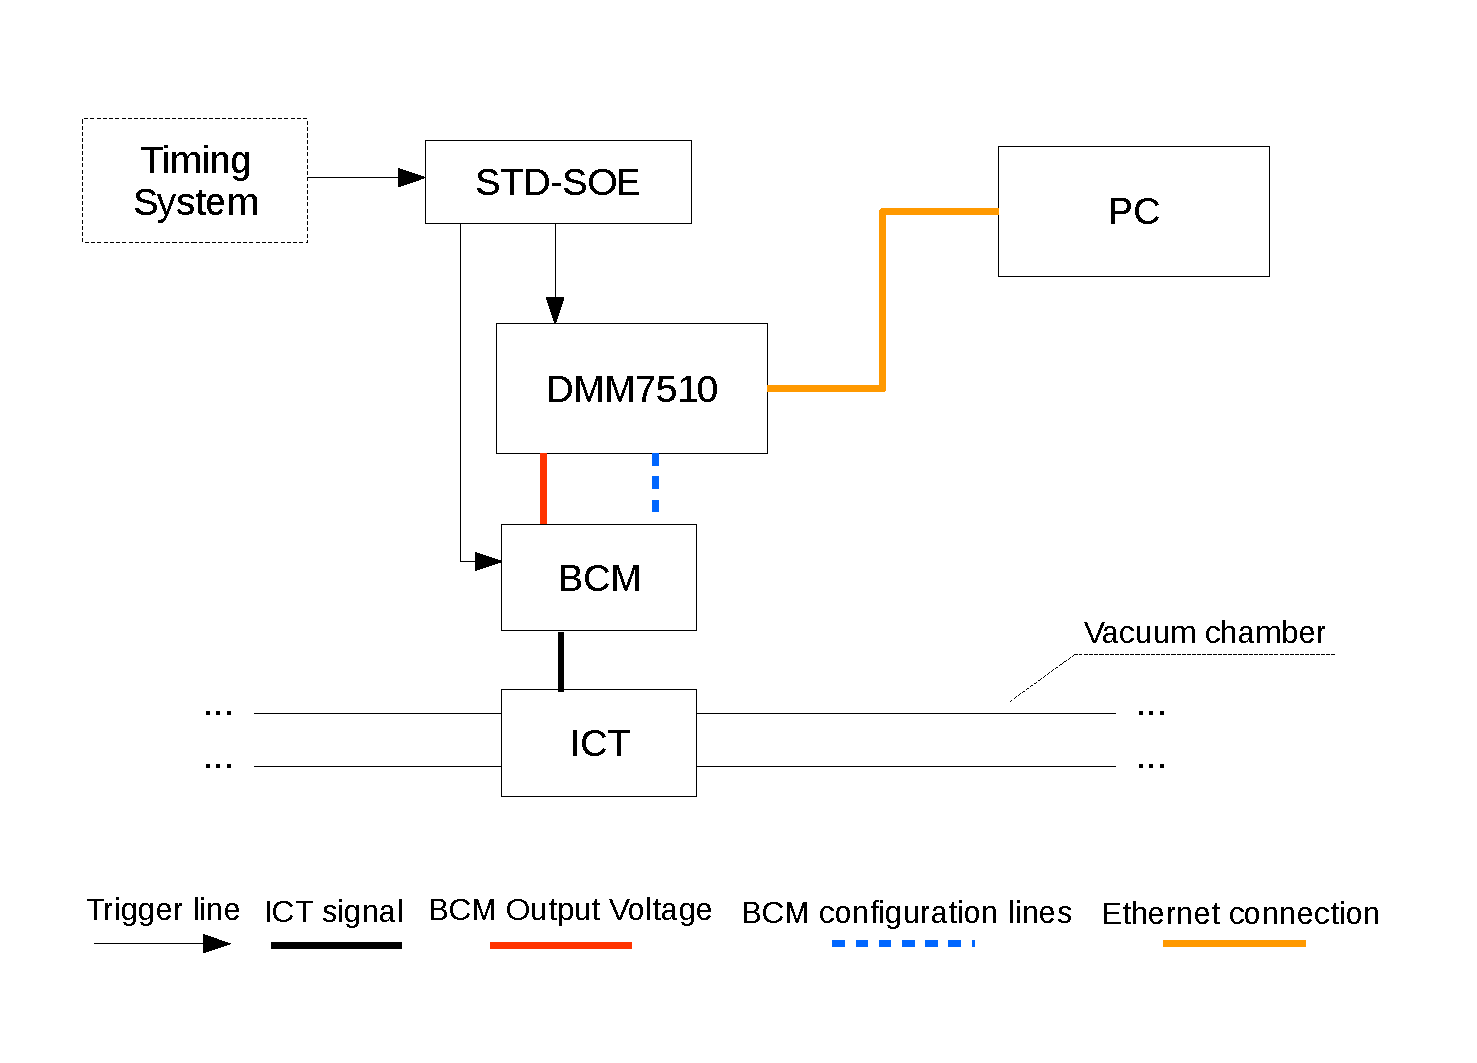
\includegraphics[width=1.0\textwidth]{ict-setup-image}
	\end{figure}
\FloatBarrier

	\paragraph{} The ICT sensor and BCM module are fabricated by Bergoz Instrumentation and used for measuring beam charge during the injection process. The ICT output signal is integrated by the BCM, which generates an output voltage level proportional to the beam pulse charge. The voltage signal is available \SI{30}{\micro\second} after the trigger and maintained up to \SI{400}{\micro\second}, then reset.

	\paragraph{} The Kethley DMM7510 digital multimeter is connected to the BCM voltage output and is used to acquire, convert, and filter the measurement data.

	\paragraph{} The STD-SOE timing module is used to trigger BCM measurements and multimeter readings.

	\paragraph{} The PC runs an EPICS IOC, which includes DMM7510 multimeter and ICT application-specific PVs. The IOC reads the multimeter data regularly and configures the multimeter's parameters according to the settings defined in the application PVs.

%--- Section: Measurement Overview ---
\section{Measurement Overview}

	\paragraph{} The beam charge measurement is triggered once each time an electron beam passes through an accelerator transport line. The Timing System is responsible for providing the measurement triggers, while the application software reads the measurement data and stores it in EPICS PVs.
	\paragraph{} There are two different trigger modes in which the multimeter can operate. The multimeter can either read and convert the BCM output signal every time an external timing trigger is received, or start a reading based on its input voltage level. When the multimeter is triggered by an external trigger, the Timing System must provide triggers for both the BCM and the multimeter. The \SI{30}{\micro\second} delay required by the BCM module before its output signal stabilizes must be added as a delay between the sensor and multimeter triggers in the Timing System configuration. When the multimeter is triggered by an input voltage level change, the Timing System is only required to provide a trigger to the BCM. BCM output signal availability is automatically detected, and after \SI{65}{\micro\second} (with high frequency rejection enabled) the multimeter reading starts.
	\paragraph{} In order to improve measurement precision, the multimeter sampling of the BCM output pulse is divided in two phases. First, as a response to the external or level based trigger, the multimeter takes a specified number of samples from the BCM pulse. Then, after \SI{16.67}{\milli\second} (interval is user-configurable) a new group of samples is taken. The measurement result is the subtraction of the averages of the first and second groups. This technique compensates zero drift due to temperature or ageing, and eliminates mains frequency noise.

	% Multimeter measurement diagram for ICT application
	\begin{figure}[!h]
		\caption{Multimeter measurement scheme for the ICT application}
		\label{fig:meas-scheme}
		\centering
		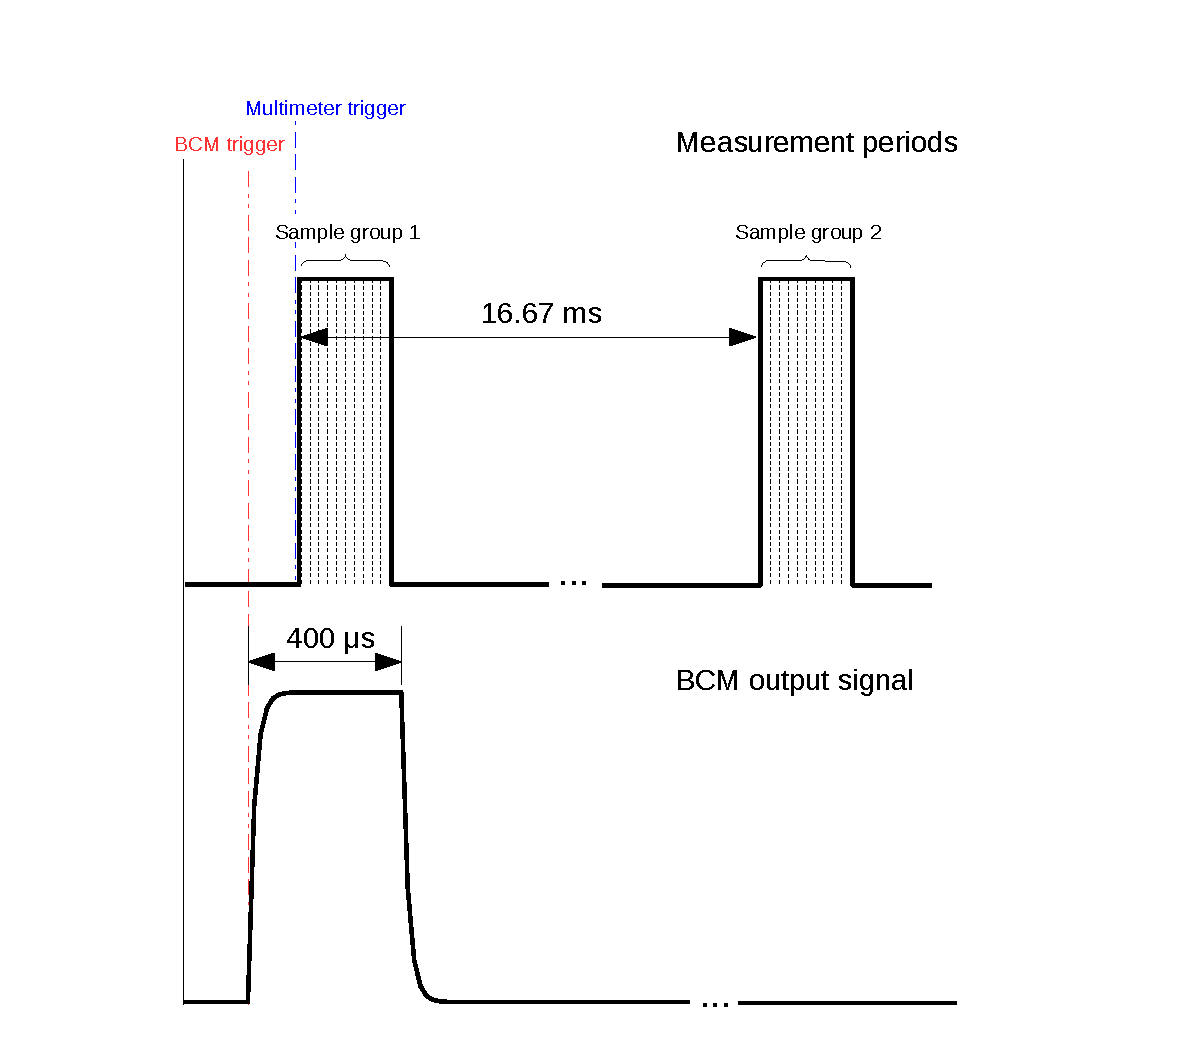
\includegraphics[width=1.0\textwidth]{ict-meas-scheme-image}
	\end{figure}
\FloatBarrier

%--- Section: ICT Software Configuration Steps ---
\section{ICT Software Configuration}

	\paragraph{} This section describes the basic steps when configuring the ICT application. Further detail about the ICT application PVs can be found in \emph{\nameref{sec:process-variables}}.

	\paragraph{} It is recommended to \hyperref[disable-triggering]{disable measurement triggering} before making any changes to the application settings and to configure triggering only after everything else has been set. This prevents incorrect measurements from being passed to any high level software by the IOC.

	\subsection{Measurement triggering}

		\paragraph{Disable triggering}\label{disable-triggering} It might be useful, in some cases, to disable measurement triggering. In this configuration, all trigger types are disabled.

			\begin{enumerate}
				\item Set \emph{DigtzeTrg-Sel} PV to \emph{None}.
				\item Wait until \emph{DigtzeTrg-Sts} has changed to \emph{None}.
			\end{enumerate}

		\paragraph{External triggering} In the external triggering mode, the DMM7510 multimeter starts measurements in response to external trigger reception. When both measurement phases have completed, the EPICS application fetchs the multimeter buffer readings.

			\begin{enumerate}
				\item Set \emph{2ndReadDly-SP} to the desired delay between first and second group of measurements. The recommended value is \emph{0.01667} (1 power line cycle).
				\item Verify if \emph{2ndReadDly-RB} value is correct.
				\item Set \emph{DigtzeTrg-Sel} PV to \emph{External}.
				\item Wait until \emph{DigtzeTrg-Sts} has changed to \emph{External}.
			\end{enumerate}

		\paragraph{Charge level based triggering} In level based triggering mode, the DMM7510 multimeter starts measurements in response to a rising edge input signal that goes above the specified threshold. The threshold is specified in nC, so that it can be easily selected considering the expected minimum charge value.

			\begin{enumerate}
				\item Set \emph{BCMRange-SP} to the BCM module full scale output voltage.
				\item Set \emph{Range-Sel} to the desired sensor measurement range.
				\item Verify if \emph{Range-Sts} has changed accordingly.
				\item Set \emph{Threshold-SP} to the threshold charge value intended to trigger measurements.
				\item Verify if \emph{Threshold-RB} has changed accordingly.
				\item Set \emph{HFReject-Sel} to indicate if high frequency rejection should be used.
				\item Verify if \emph{HFReject-Sts} has changed accordingly.
				\item Set \emph{DigtzeTrg-Sel} to \emph{InLevel}.
				\item Wait until \emph{DigtzeTrg-Sts} has changed to \emph{InLevel}.
			\end{enumerate}

	\subsection{BCM Range selection}

		\paragraph{} The selected BCM range determines the sensor sensitivity.

			\begin{enumerate}
				\item Set \emph{BCMRange-SP} to the full scale output voltage of the BCM module.
				\item Set \emph{Range-Sel} to the desired sensor measurement range.
				\item Verify if \emph{Range-Sts} has changed accordingly.
			\end{enumerate}

	\subsection{Measurement settings}

		% Measurement characteristcs figure
		\begin{figure}[!h]
			\caption{Measurement parameters}
			\label{fig:meas-param}
			\centering
			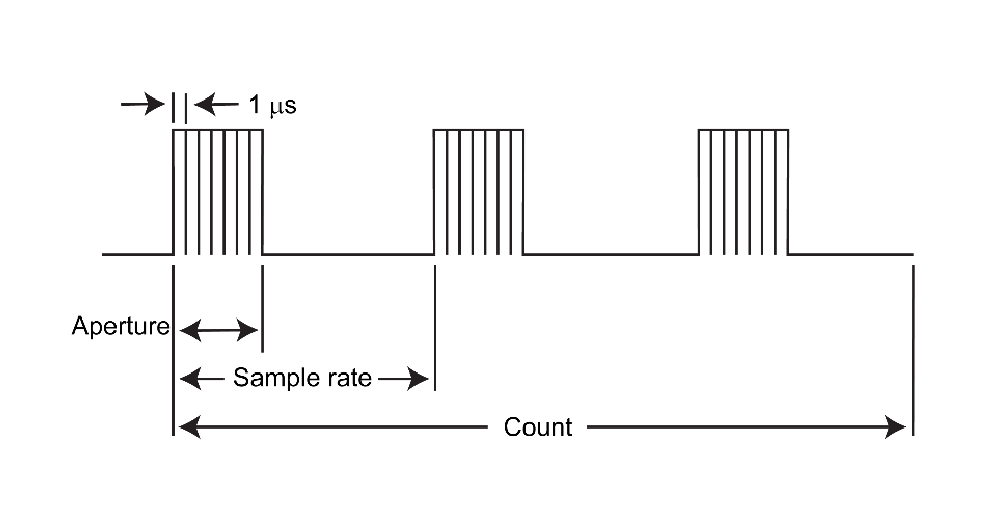
\includegraphics[width=1.0\textwidth]{ict-meas-param-image}
		\end{figure}
\FloatBarrier

		\paragraph{} A few parameters are responsible for defining the measurement characteristics.

			\begin{enumerate}
				\item \emph{DigtzeCount-SP} sets the number of samples taken during each measurement phase. In total, $ 2\times count $ measurements are taken, first half just after the trigger, and second half one power line cycle later.
				\item \emph{DigtzeCount-RB} indicates the configured number of measurements per measurement phase.
				\item \emph{Aperture-SP} sets the measurement integration period in \SI{}{\micro\second}.
				\item \emph{Aperture-RB} indicates the configured integration period in \SI{}{\micro\second}.
				\item \emph{SampleRate-SP} sets the sampling rate of measurements. Indirectly determines the interval between samples.
				\item \emph{SampleRate-RB} indicates the configured measurement sampling rate.
				\item \emph{Imped-Sel} sets the multimeter's input impedance. The recommended setting is \emph{AUTO}.
				\item \emph{Imped-Sts} indicates the configured multimeter's input impedance.
			\end{enumerate}

	\subsection{BCM calibration}

		\paragraph{} The BCM module has a calibration generator that can be used for on-line calibration.

			\begin{enumerate}
				\item \emph{CalEnbl-Sel} enables/disables the BCM calibration generator.
				\item \emph{CalEnbl-Sts} indicates the BCM calibration generator status.
				\item \emph{CalCharge-Sel} sets the calibration pulses charge. This is charge as applied to the input of the Charge Amplifier. It is not beam pulse charge equivalent.
				\item \emph{CalCharge-Sts} indicates the calibration pulses charge status.
			\end{enumerate}

	\subsection{Save function}

		\paragraph{} The save function stores the current PV configurations and restore them when the IOC is restarted.

			\begin{enumerate}
				\item Set \emph{Save-Cmd} to \emph{ON} to cause the \emph{-SP} and \emph{-Sel} PVs' values to be saved. During IOC startup, the saved PV values are restored, recovering the previous configuration.
			\end{enumerate}

%--- Section: Reading Measurements from PVs ---
\section{Reading Measurements from PVs}

	\paragraph{} The ICT measurement data is available in the following EPICS PVs.

		\begin{enumerate}
			\item \emph{Charge-Mon} stores the latest filtered charge measurement.
			\item \emph{ChargeHstr-Mon} is a circular buffer storing the last 1000 filtered measurements.
			\item \emph{RawReadings-Mon} is an array containing the lastest measurement raw data, i.e., $ 2 \times count $ readings, in which the first and second halves correspond, respectively, to the first and second phases of the measurement.
			\item \emph{RawPulse-Mon} is an array containing the first half of \emph{RawReadings-Mon}, i.e., raw data corresponding to measurements taken during the BCM pulse.
			\item \emph{RawNoise-Mon} is an array containing the second half of \emph{RawReadings-Mon}, i.e., raw data corresponding to measurements taken after the BCM pulse, during the second measurement phase.
		\end{enumerate}

\section{Process Variables Description}\label{sec:process-variables}

	% Process Variables description table
	\begin{longtable}{| m{3.0cm} m{4.5cm} m{7.0cm} |}
		\caption{Application Process Variables} \\ \hline
		\bfseries Name & \bfseries Data Type & \bfseries Description \label{tab:PV-description} \endfirsthead
		\caption{Application Process Variables} \\ \hline
		\bfseries Name & \bfseries Data Type & \bfseries Description \endhead \hline
		% --- row ---
		Charge-Mon & FLOAT: 32-bit & \begin{tabular}{@{}m{6cm}@{}}
	    					Latest charge measurement. This PV holds the measurement produced by filtering the latest multimeter readings.
						\end{tabular} \\ \hline
		% --- row ---
		ChargeHstr-Mon & FLOAT[1000] & \begin{tabular}{@{}m{6cm}@{}}
	    					Last 1000 charge measurements. This PV is a circular buffer holding the last 1000 filtered charge measurements.
						\end{tabular} \\ \hline
		% --- row ---
		RawReadings-Mon & FLOAT[1000] & \begin{tabular}{@{}m{6cm}@{}}
	    					Latest measurement raw data. This PV holds the raw data used when computing the latest measurement. The PV stores $ 2 \times count $ readings, in which the first and second halves correspond, respectively, to the first and second phases of the measurement.
						\end{tabular} \\ \hline
		% --- row ---
		RawPulse-Mon & FLOAT[1000] & \begin{tabular}{@{}m{6cm}@{}}
	    					First half of \emph{RawReadings-Mon} array. This PV holds the raw data corresponding to the first measurement phase, which is the data acquired during the BCM pulse. The first measurement phase contains $count$ readings.
						\end{tabular} \\ \hline
		% --- row ---
		RawNoise-Mon & FLOAT[1000] & \begin{tabular}{@{}m{6cm}@{}}
	    					Second half of \emph{RawReadings-Mon} array. This PV holds the raw data corresponding to the second measurement phase, which is the data acquired after the BCM pulse after \emph{2ndReadDly-SP} seconds, and used for noise rejection. The second measurement phase contains $count$ readings.
						\end{tabular} \\ \hline
		% --- row ---
		DigtzeTrg-Sel & ENUM: None, External, InLevel & \begin{tabular}{@{}m{6cm}@{}}
				      	  Digitize trigger source. When set to \emph{External}, the multimeter measurements are triggered by an external trigger. When set to \emph{InLevel}, measurements are triggered when the input signal exceeds the specified threshold (rising edge transition). For both \emph{External} and \emph{InLevel} triggering, the software fetchs $ 2 \times count $ readings from the multimeter's buffer as soon as they are available.
					  \end{tabular} \\ \hline
		% --- row ---
		DigtzeTrg-Sts & ENUM: Unknown, External, InLevel, None & \begin{tabular}{@{}m{6cm}@{}}
	    					Trigger source selection status.
						\end{tabular} \\ \hline
		% --- row ---
		Range-Sel & ENUM: 40 nC, 20 nC, 10 nC, 8 nC, 4 nC, 2 nC, 0.8 nC & \begin{tabular}{@{}m{6cm}@{}}
	    					BCM range selection.
						\end{tabular} \\ \hline
		% --- row ---
		Range-Sts & ENUM: 40 nC, 20 nC, 10 nC, 8 nC, 4 nC, 2 nC, 0.8 nC & \begin{tabular}{@{}m{6cm}@{}}
	    					BCM range selection status.
						\end{tabular} \\ \hline
		% --- row ---
		2ndReadDly-SP & FLOAT: Min=0.000008, Max=100000 & \begin{tabular}{@{}m{6cm}@{}}
	    					Second reading phase delay. The second reading phase delay specifies, in seconds, the delay between the external or level based trigger and the second group of measurements start.
						\end{tabular} \\ \hline
		% --- row ---
		2ndReadDly-RB & FLOAT: Min=0.000008, Max=100000 & \begin{tabular}{@{}m{6cm}@{}}
	    					Second reading phase delay readback value.
						\end{tabular} \\ \hline
		% --- row ---
		Threshold-SP & FLOAT: Min=0, Max=40 & \begin{tabular}{@{}m{6cm}@{}}
	    					Beam charge threshold. When level based triggering is selected, multimeter readings start on input signal rising edge transitions that go above the specified charge threshold.
						\end{tabular} \\ \hline
		% --- row ---
		Threshold-RB & FLOAT: Min=0, Max=40 & \begin{tabular}{@{}m{6cm}@{}}
	    					Beam charge threshold readback value.
						\end{tabular} \\ \hline
		% --- row ---
		HFReject-Sel & BOOL: OFF, ON & \begin{tabular}{@{}m{6cm}@{}}
	    					Enable/disable high frequency rejection. When enabled, high frequency rejection requires the signal to remain above the specified threshold for at least \SI{64}{\micro\second} before a trigger is generated. This paremeter affects the level based measurement trigger.
						\end{tabular} \\ \hline
		% --- row ---
		HFReject-Sts & BOOL: OFF, ON & \begin{tabular}{@{}m{6cm}@{}}
	    					High frequency rejection enable status.
						\end{tabular} \\ \hline
		% --- row ---
		BCMRange-SP & FLOAT: Min=1, Max=10 & \begin{tabular}{@{}m{6cm}@{}}
	    					BCM full scale output range. This value is used by conversion calculations.
						\end{tabular} \\ \hline
		% --- row ---
		DigtzeCount-SP & LONG: Min=1, Max=1000000 & \begin{tabular}{@{}m{6cm}@{}}
	    					Digitize count. Number of samples taken during each measurement phase. Along with the digitize sample rate, determines the duration of the measurement phases.
						\end{tabular} \\ \hline
		% --- row ---
		DigtzeCount-RB & LONG: Min=1, Max=1000000 & \begin{tabular}{@{}m{6cm}@{}}
	    					Digitize count readback value.
						\end{tabular} \\ \hline
		% --- row ---
		Aperture-SP & LONG: Min=1, Max=1000 & \begin{tabular}{@{}m{6cm}@{}}
	    					Digitize aperture. Duration of each sample's integration period in \SI{}{\micro\second}.
						\end{tabular} \\ \hline
		% --- row ---
		Aperture-RB & LONG: Min=1, Max=1000 & \begin{tabular}{@{}m{6cm}@{}}
	    					Digitize aperture readback value.
						\end{tabular} \\ \hline
		% --- row ---
		SampleRate-SP & LONG: Min=1000, Max=1000000 & \begin{tabular}{@{}m{6cm}@{}}
	    					Digitize sample rate. Indirectly determines the interval between samples and, along with the digitize count, the duration of the measurement phases.
						\end{tabular} \\ \hline
		% --- row ---
		SampleRate-RB & LONG: Min=1000, Max=1000000 & \begin{tabular}{@{}m{6cm}@{}}
	    					Digitize sample rate readback value.
						\end{tabular} \\ \hline
		% --- row ---
		Imped-Sel & BOOL: AUTO, 10MOhm & \begin{tabular}{@{}m{6cm}@{}}
	    					Multimeter input impedance. Selecting \emph{AUTO} optimizes for low noise and charge injection when the device under test has less than \SI{100}{\kohm} input resistance. Otherwise, \emph{10MOhm} optimizes for lowest noise.
						\end{tabular} \\ \hline
		% --- row ---
		Imped-Sts & BOOL: AUTO, 10MOhm & \begin{tabular}{@{}m{6cm}@{}}
	    					Multimeter input impedance status.
						\end{tabular} \\ \hline
		% --- row ---
		CalEnbl-Sel & BOOL: OFF, ON & \begin{tabular}{@{}m{6cm}@{}}
	    					Enable/disable BCM calibration generator. When the BCM calibration generator is enabled, the BCM module generates two calibration pulses with opposite polarity right after a trigger is received by the module.
						\end{tabular} \\ \hline
		% --- row ---
		CalEnbl-Sts & BOOL: OFF, ON & \begin{tabular}{@{}m{6cm}@{}}
 						BCM calibration generator enable status.
						\end{tabular} \\ \hline
		% --- row ---
		CalCharge-Sel & BOOL: OFF, ON & \begin{tabular}{@{}m{6cm}@{}}
	    					BCM calibration charge. This is charge as applied to the input of the Charge Amplifier. See the BCM Manual for beam charge equivalents.
						\end{tabular} \\ \hline
		% --- row ---
		CalCharge-Sts & BOOL: OFF, ON & \begin{tabular}{@{}m{6cm}@{}}
 						BCM calibration charge status.
						\end{tabular} \\ \hline
		% --- row ---
		Save-Cmd & BOOL: OFF, ON & \begin{tabular}{@{}m{6cm}@{}}
 						Save command. When set to \emph{ON}, this PV causes all \emph{-SP} and \emph{-Sel} PVs values to be saved. During IOC initialization, the saved PV values are restored.
						\end{tabular} \\ \hline
		% --- row ---
		Download-Cmd & BOOL: OFF, ON & \begin{tabular}{@{}m{6cm}@{}}
 						Download command. When set to \emph{ON}, this PV causes all \emph{-SP} and \emph{-Sel} PVs' values to be transferred to hardware. This PV is set automatically during IOC initialization and when the IOC recovers from a communication problem with the hardware.
						\end{tabular} \\ \hline

	\end{longtable}

\end{document}
\grid
